\chapter{State of the Art: Optimal path planning for autonomous robots}

\renewcommand{\chaptername}{Chapter}

\section*{Introduction}
This chapter focuses on a sythesis of the literature around Optimal Near-field Path planning
for robots in Intralogistics environments. 
It starts with an explanation of the fundamemental aspects this work is based on 
as Automated Mobile Robots (AMRs), Near-field Path planning and Optimization techniques 
with a focus on Intralogistics.
Then it focuses on the path planning approaches proposed to rise to the existing challenges.
Later, the topic of optimization is outlined, investigating the decision-making science
that leads to the elimination of some path planning drawbacks.
It concludes with a discussion around which works from the literature can be used for this problem 
statement and how they can be exploited for this work.

\section{Intralogistics Environments}
Intralogistics refers to the management, control, and optimization of internal material and 
information flow within a warehouse \Ref{R28}. It encompasses all physical and operational processes 
involved in the movement of materials and goods. This concept was introduced and defined by 
the German Engineering Association (VDMA). Figure \Ref{Areas} covers various aspects of 
intralogistics areas, including 
the storage, transportation, supply, Manufacturing, and disposal of production materials, as well as 
shipping. 
The scope of this work is focused around the warehouse 
area where storage: picking, and placing, takes place. 
In brownfield applications, introduced in the General Introduction, the warehouse environment is 
usually a crowded and cluttered 
atmosphere: The nature of activities like manufacturing storing installs a high level of 
dynamics, whether it is operators or other vehicles, and obstacles as boxes and pallets. 
The cluttered 
and highly dynamic nature of this environment makes it challenging to successfully 
implement robotic based solutions.

\begin{figure}[H]
    \begin{center}
        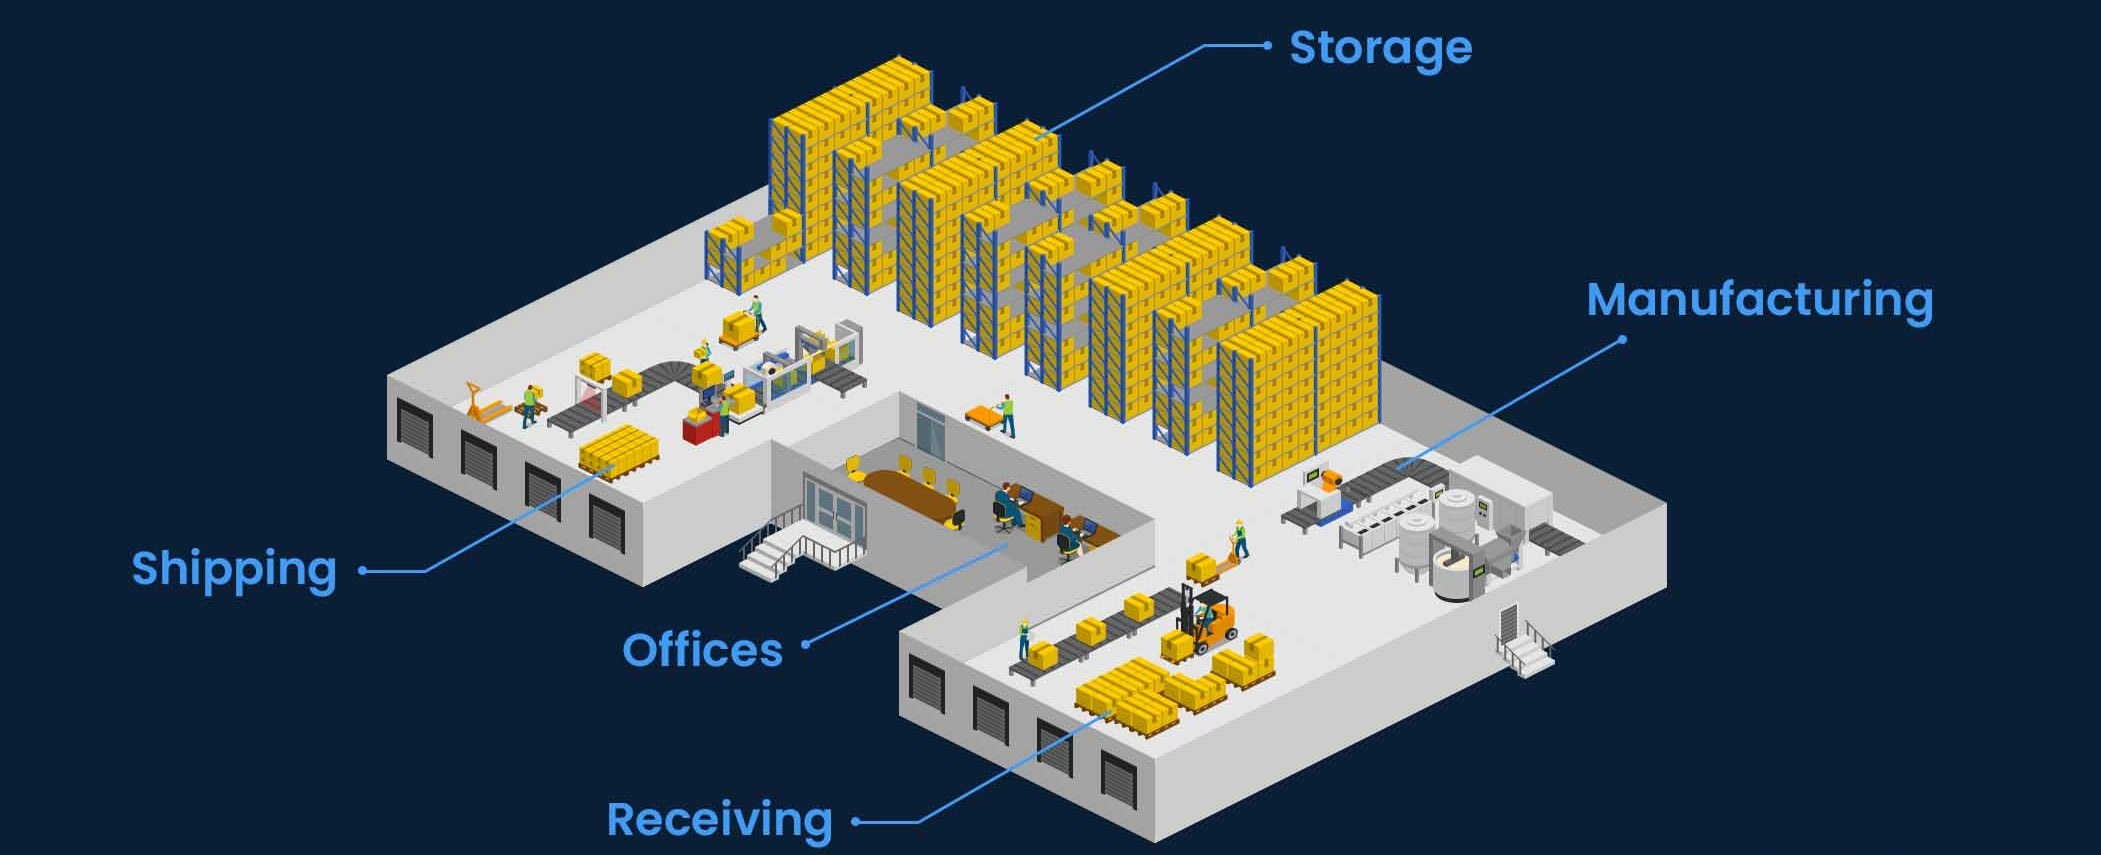
\includegraphics[width=6in]{images/Chap1/common-warehouse-areas.jpg}\\
        \caption{Common Intralogistics Environment Areas \cite{R46}}
        \label{Areas}
        \end{center}
\end{figure}

\section{AMRs in Intralogistics Environments}
Autonomous Mobile Robots (AMRs) are advanced robots designed to navigate and perform tasks independently 
in dynamic environments without the need for fixed infrastructure or human intervention. Equipped with 
sensors, cameras, and advanced software, AMRs can move around facilities like warehouses and 
factories, adjusting their paths based on real-time conditions. They are commonly used 
for material handling and transporting goods \cite{R7}.

AMRs are a type of non-holonomic vehicles. Non-holonomic vehicles are systems whose movement is subject 
to constraints that limit their ability to move freely in all directions. Specifically, their constraints 
depend on their configuration and velocities, meaning they cannot instantaneously move in certain directions 
(e.g., sideways), but must follow a specific path or series of movements to achieve certain positions. 
This contrasts with holonomic systems, which can move in any direction directly without such constraints \cite{R28}.

In the Intralogistics field, AMRs were introduced as a revolution to Automated Guided Vehicles (AGVs) \cite{R7}. 
First introduced in 1955, AGVs performed tasks like 
material handling. AGVs are managed by top-level software that handles task planning, 
providing the vehicles with intermediate waypoints to navigate from start to end points \cite{R7}.
On the other hand, AMRs are automated in a way that makes them find the solution to unexpected problems, 
in fact:
Figure \Ref{AMR-VS-AGV}, shows the difference in behavior between an AMR and an AGV in the case of a 
new obstacle. While AMRs are able to surpass the obstacle through sensors recognition and obstacle 
avoidance algorithms, AGVs require human intervention to eliminate the obstacle before restarting the navigation.

AMRs fit in the cluttered ares of warehouses. Their perception of the surrounding information allows for
low commissioning efforts: they are able to localize themselves, plan then navigate to the goal and reach their 
destinations autonomously. Their operation does not require an expert or an engineer's intervention which 
limits the commissioning and utilization costs.

\begin{figure}[H]
    \begin{center}
       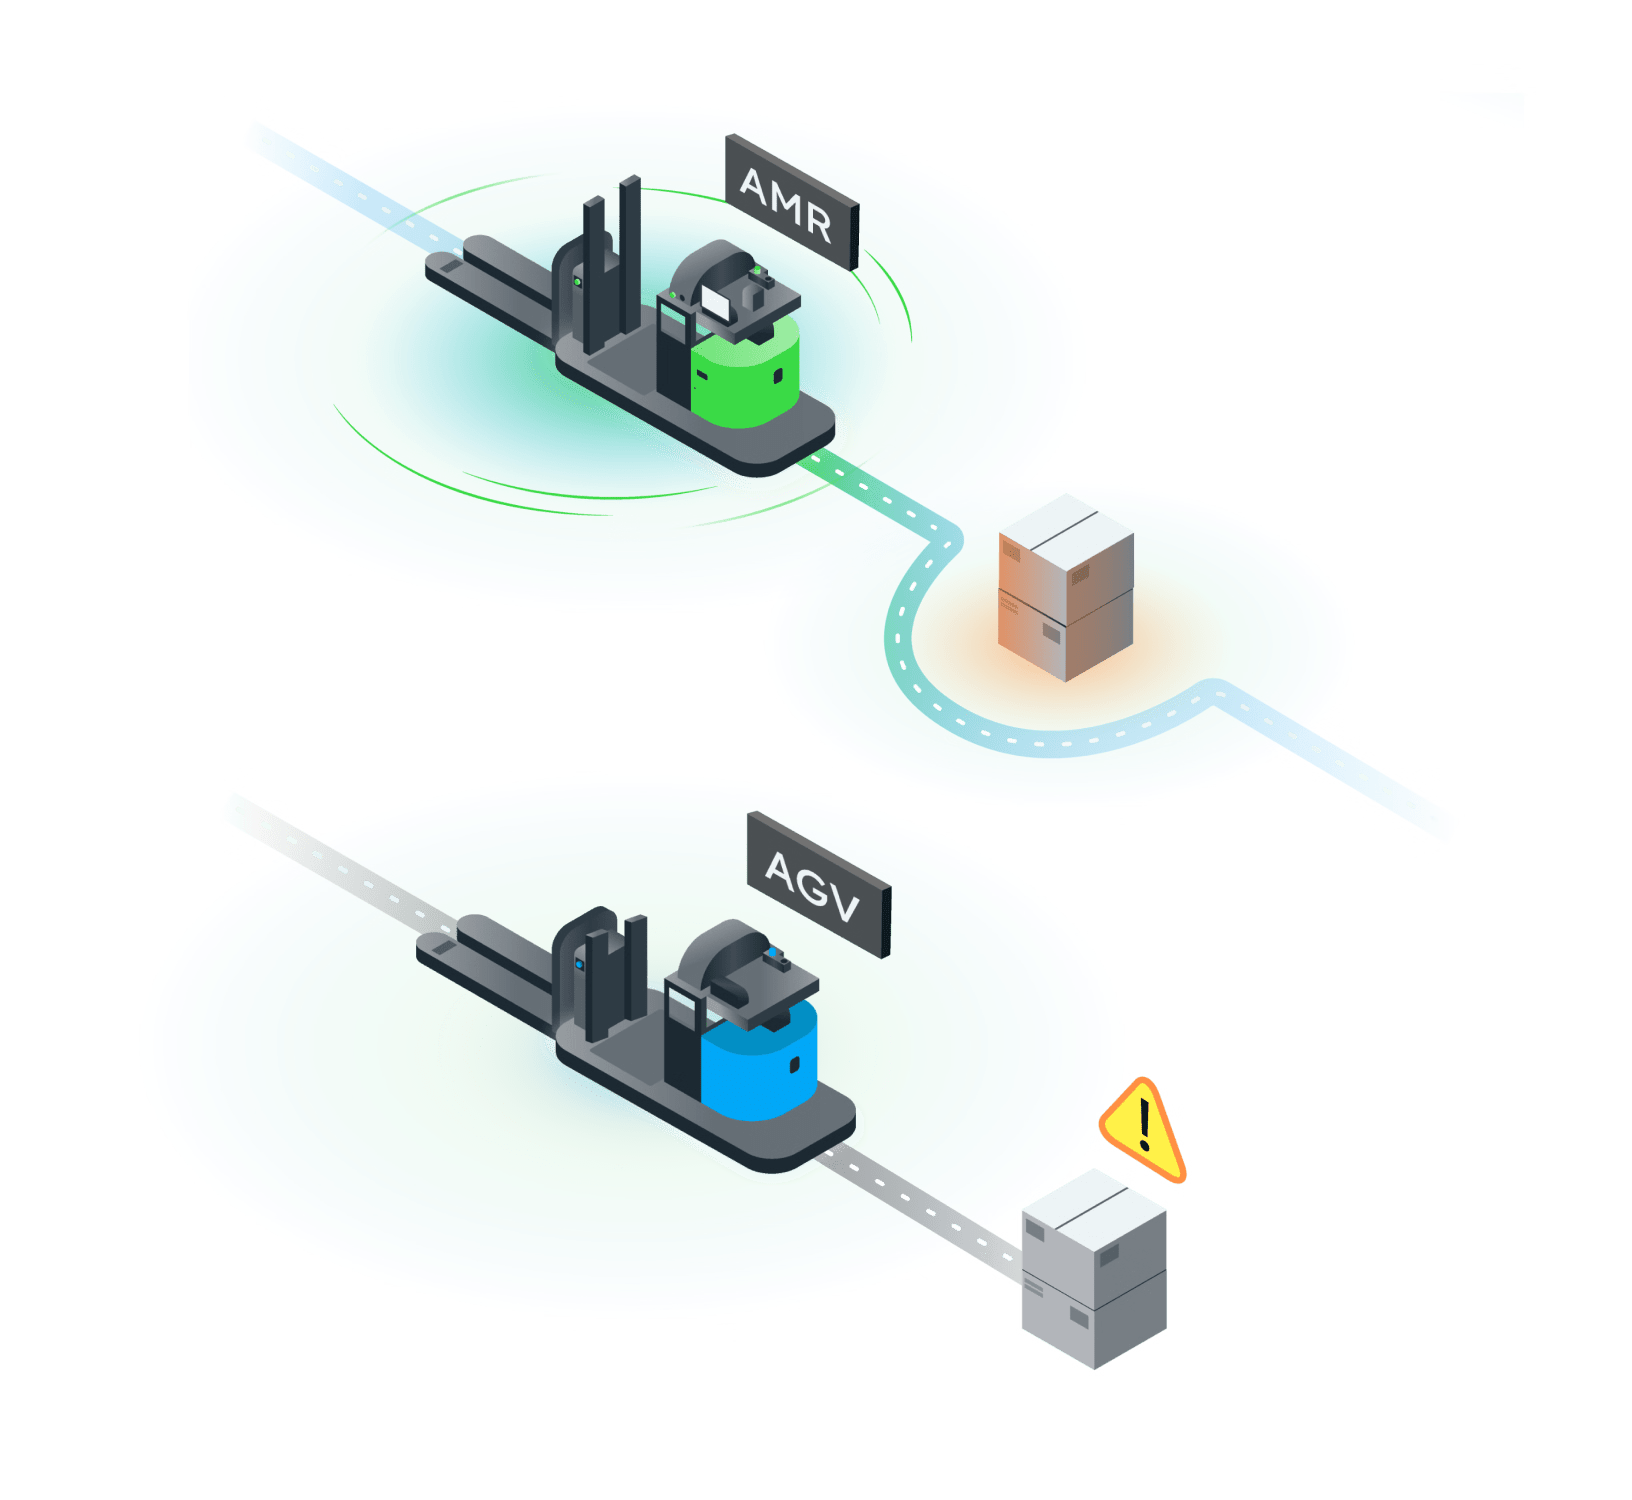
\includegraphics[width=4in]{images/Chap1/AMR-VS-AGV.png}\\
       \caption{AMR and AGV behaviors at presence of an obstacle \cite{R9}}
       \label{AMR-VS-AGV}
       \end{center}
\end{figure}

%\begin{figure}[H]
%    \begin{center}
%       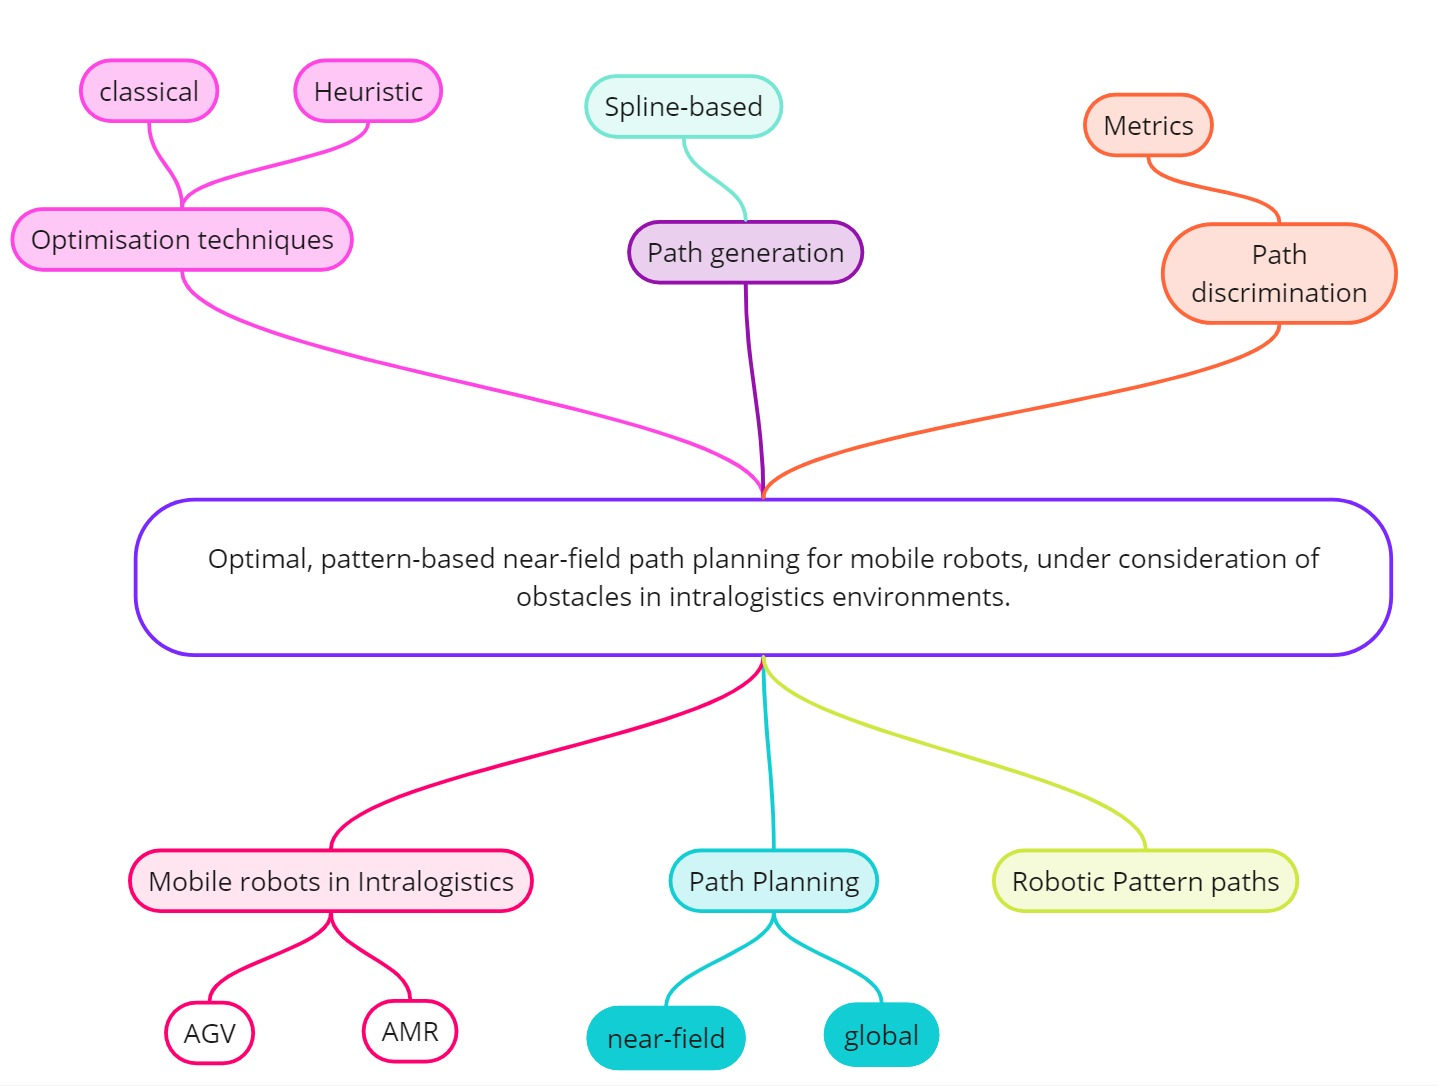
\includegraphics[width=5in]{images/Chap1/Fig1.jpg}\\
%       \caption{Mind map of the key topics}
%       \label{mindmap}
%       \end{center}
%\end{figure}

\section{Path Planning}
This section will dive into the path planning state of the art: outlining its promising 
opportunities and current challenges, detailing the different approaches, and discussing
%how to employ their efficienyćy for this 
their efficiency and compatibility with the problem statement.

\subsection{Path Planning for autonomous robots: Opportunities and challenges}
%opportunities
Path planning for mobile robots involves creating and generating efficient routes 
for the robot to travel from a starting position (A) to a target position (B), 
ensuring minimal time and travel distance while avoiding collisions with nearby objects \cite{R7}. Literature 
differentiates between two main types of path planning: 
global and local path planning \cite{R11}. Global planning involves finding an optimal path from 
the start to the target position based on sensor input within a known, static environment, 
whereas local planning focuses on real-time path planning and obstacle avoidance, typically used online while 
moving to avoid dynamic obstacles \cite{R11}.

In complex environments, movement and task fulfillment must be done carefully and accurately given 
the volume of the vehicle and the value of the handled material. With appropriate input from various sensors, 
such as laser 
scanners, cameras, and LiDAR providing robots can perceive of their surrounding environment and plan the right path
accordingly. This hardware innovation made navigation flexibility and autonomous recovery 
after failure possible\cite{R7}.
The relevance of efficient path planning, mainly in the intralogistics sector, is derived from the constant need 
of optimizing material flow, productivity rates, and cost effectiveness. Path planning reduces
travel time and distances when moving goods and thus , improving overall operational costs by allowing robots 
to take the most optimal routes when moving goods. By minimizing unnecessary detours and avoiding congested areas, 
robots can complete tasks more quickly, leading to faster material handling cycles.
In those dynamic environments (see chapter 2, section 1), operators and employees are moving around, 
goods and pallets are 
being transported or stocked, and materials must be handled safely and carefully.
Flexibility in routing and planning, enables the AMRs to always drive the optimal path
based on the space settings. This flexibility offers several benefits, such as:

\begin{itemize}
    \item Independence from Human intervention if an unexpected situation raises 
    -AMRs do not require assistance, unike AGVs \cite{R7}.
    \item Reduced energy consumption thanks to optimal, smooth and short paths that adhere to 
    the vehicles' kinematics, allocated task and travel time.
    \item Robustness and responsiveness thanks to decentralized decison making: enables fast 
    recovery and change of strategy after failure\cite{R7}.
\end{itemize}

Efficient path planning is critical for ensuring safe and reliable handling of objects in dynamic environments. 
By maintaining safe distances from both static and moving obstacles, including people, and continuously detecting 
surroundings, robots can ensure safety at all times. An optimized path improves both the length and 
smoothness of travel, minimizing travel time and boosting productivity, as tasks are repeated frequently 
throughout the day. As a result, it enhances operational efficiency, contributing to overall system 
performance.

AMRs, as the name suggests, are 
standalone systems that must compile and process such input and generate, through algorithms, 
efficient paths. Path planning serves as the crucial 
link between the robot’s sensor input and its motion control \cite{R10}.


%challenges 
%Todo: add reference for 
More that 60 years have elapsed since "Shaky" the first wheeled robot was running it first tests
in Stanford University' labs. However, most of the robotic related topic are still being researched and improved.
Dealing with all the aspects and challenges that robotics comes with can be very intricate. One of the major 
topics posing challenges to researchers is path planning. 
In \cite{R20}, authors reviewed recent path planning approaches and challenges
in dynamic unkown environments. 
% safety
Saftey in path planning was the main concern for 29 \% of the reviewed studies. Navigating efficient 
paths while avoiding collisions is challenging to accomplish. Collision avoidance is tightly related to perception 
input through sensors, analysis and use of the data. While it may seem simple for the robots to correctfully analyze 
and recognize the objects around them, in reality, detailed understanding is not possible \cite{R21}. Issues are 
related to the accuracy of the sensors and the robustness of the algorithms. 
It is expected from the robot to 
preceive of the obstacles just like humans do, recognizing 3d shapes, dimensions, depth, direction and velocity, 
but from the 
robot's perspective, it is only able to recognize the outer surface that reflects the sensor's luminous signals. As shown in
figure \Ref{scamSim}, the simulated robot (in gray) is surrounded by 3 obstacles (blue polygons).
While the obstacles are polygon-shaped, the perception of the robot is limited to the surfaces that 
it can scan and does not see the hidden depth beyond these surfaces.

\begin{figure}[H]
    \begin{center}
        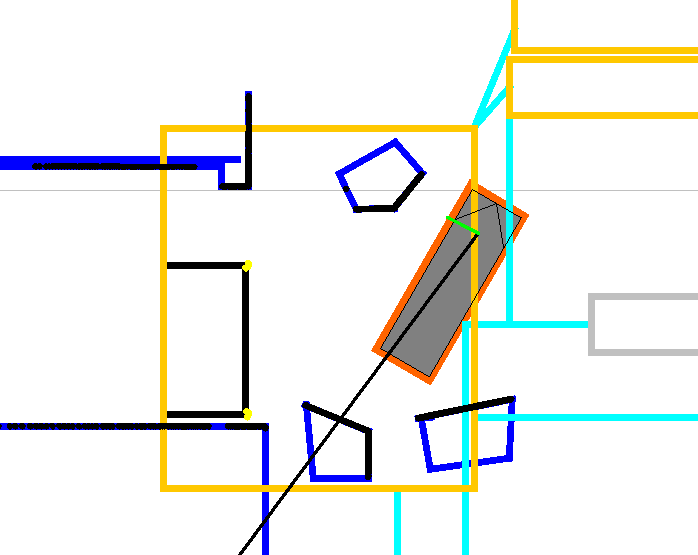
\includegraphics[width=4in]{images/Chap1/scan.png}\\
        \caption{
        Simulation of the robot's perception of surrounding obstacles.
        \newline \textbf{Yellow rectangle:} Station limits
        \newline \textbf{Black rectangle:} Shelf limits: where to pick or to place pallets
        \newline \textbf{In gray:} Robot in simulation
        \newline \textbf{Blue polygones:} Simulated obstacles
        \newline \textbf{Black lines:} Perceived obstacle points}
        \label{scamSim}
        \end{center}
\end{figure}

As a result, algorithms are to compensate the shadowed depth of obstacles by enforcing safety measures like 
keeping the vehicle at a safe distance from the obstacles and deccelerating at the proximity 
of static and dynamic objects to avoid collisions \Ref{R28}.
In addition, this input contains noises caused by the sensors reflections of other objects
or inaccuracies \Ref{R28}. 
This makes it challenging to interpret the input and create deliberative systems as the built algorithms have to 
deal with the given data
in all cases and detect the inaccuracies and noises.
Beyond that, it is complex to generate feasible solutions in all types of environments,
some planners and algorithms risk stagnating in a local minima and not converging to the optimal routes
due to the limited knowledge of the environment and the sensory limitations previously mentioned \Ref{R28}. 
Figure \Ref{local_minima} shows a simplified example of a potential wrong decision. A vehicle encounters two possible 
driving paths, similar to what might happen in a racking system. Based solely on sensor data 
(grey shaded area), the correct path cannot be determined. Only with global path planning (green path) 
can a long-term route be selected (black arrow), avoiding the risk of ending up in a dead end (red arrow). 
Assuming the global trajectory leads to the mission goal, any local deviations from this path should be 
kept minimal while avoiding obstacles.

\begin{figure}[H]
    \begin{center}
        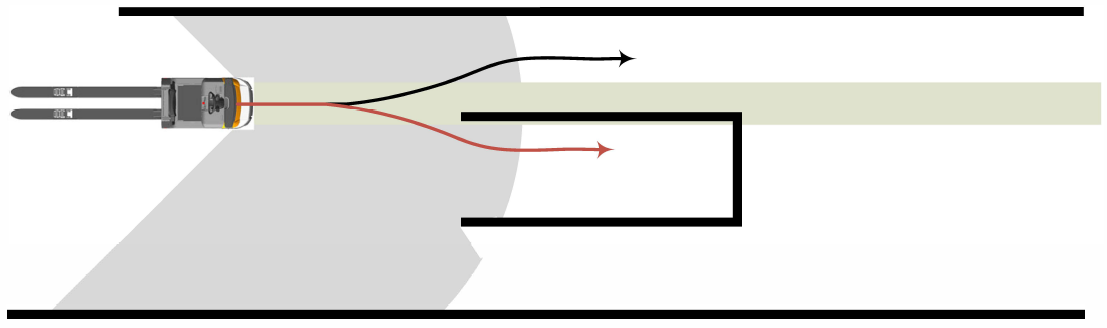
\includegraphics[width=4in]{images/Chap1/local_minima.png}\\
        \caption{Model of a local minima problem 
        due to limited sensor output \cite{R28}}
        \label{local_minima}
        \end{center}
\end{figure}

%Computational intensivity

Besides safety, computational cost is an interesting topic that researches 
are looking at. In a real time context, it is important to synchronize different tasks, 
analyze massive amounts of data generated by sensors and camera like point clouds and 2d/3d images, 
and compute the required decisions in a reliable and accurate way. As the complexity of the environment 
increases, so does the computational burden, often leading to longer processing times or the need for 
more powerful hardware \cite{R23}.

%smooth paths length and control:
While managing computational costs is crucial, it is equally important to ensure that the paths 
generated are not only computationally efficient but also smooth and short, as these factors 
significantly influence the robot's overall performance.
Given the kinematics of a robot, the destination's location and the clutter in the environment, 
path planners usually render rough paths. Cusps, which are sudden and sharp direction changes, and high
curvatures of the path are unusual path properties that are hard to drive, energy and time inefficient, 
and require continuous decelerations and accelerations. Long paths are also not favored. While they can be 
necessary to avoid obstacles or to create a smooth path, longer distances result in time consumption and 
extensive energy usage. 
Some path planner include post-smoothing methods that modify the paths after its creation and intervene by
shortening and smoothing paths areas while obstacles. In \cite{R23}, Heiden et al. present approaches 
to implement post-smoothing methods like B-Splines, Shortcuts, Simplify Max, and vertex optimization. 
They conclude that different methods deal with certain 
improvements areas differently. For example, While Splines are outperformed in the curvature and cusps 
areas, they are efficient when it comes to path-smoothning computation time.  

In conclusion, tackling robot path planning requires looking at several improvement
areas: computational intensivity, smoothing, and safety at the same time. Most path planning approaches 
are effective in the aspects that they focus on, but lack optimization in others. This further emphasizes that these 
challenges remain under research and are not yet fully addressed in the literature. While these challenges 
highlight areas needing further exploration, path planning approaches propose techniques 
to address them. Understanding these approaches can provide insights into potential solutions and 
advancements in overcoming the existing limitations.


\subsection{Near-Field Path Planning}
Path planning can be differentiated into Global Path Planning (GPP) and Local
Path Planning (LPP) or Near-Field Path Planning (NFPP). The GPP generates a global trajectory based on static and 
known environment model, such as the current pose, target location and the static components 
of the environment like shelves and walls \cite{R28}. 
The LPP generates relative trajectories and allows deviation from the previously generated global 
trajectory if disturbances in the travel path are detected. However, LPP tend to converge into local 
minima as explained in the previous section .

Due to the sheer number of publications around LPP, the work of  Kr\"uger-Basjmeleh \cite{R28} clusters 
processes into 4 groups. Figure \Ref{cluster} illustrates 4 clusters. 
The classification of the methods is done by dividing them into direction, speed, and path generating methods and 
other methods based on AI for NFPP. All methods rely equally on immediate sensory input from the 
environment as the basis for future tracking strategies.

\begin{figure}[H]
    \begin{center}
        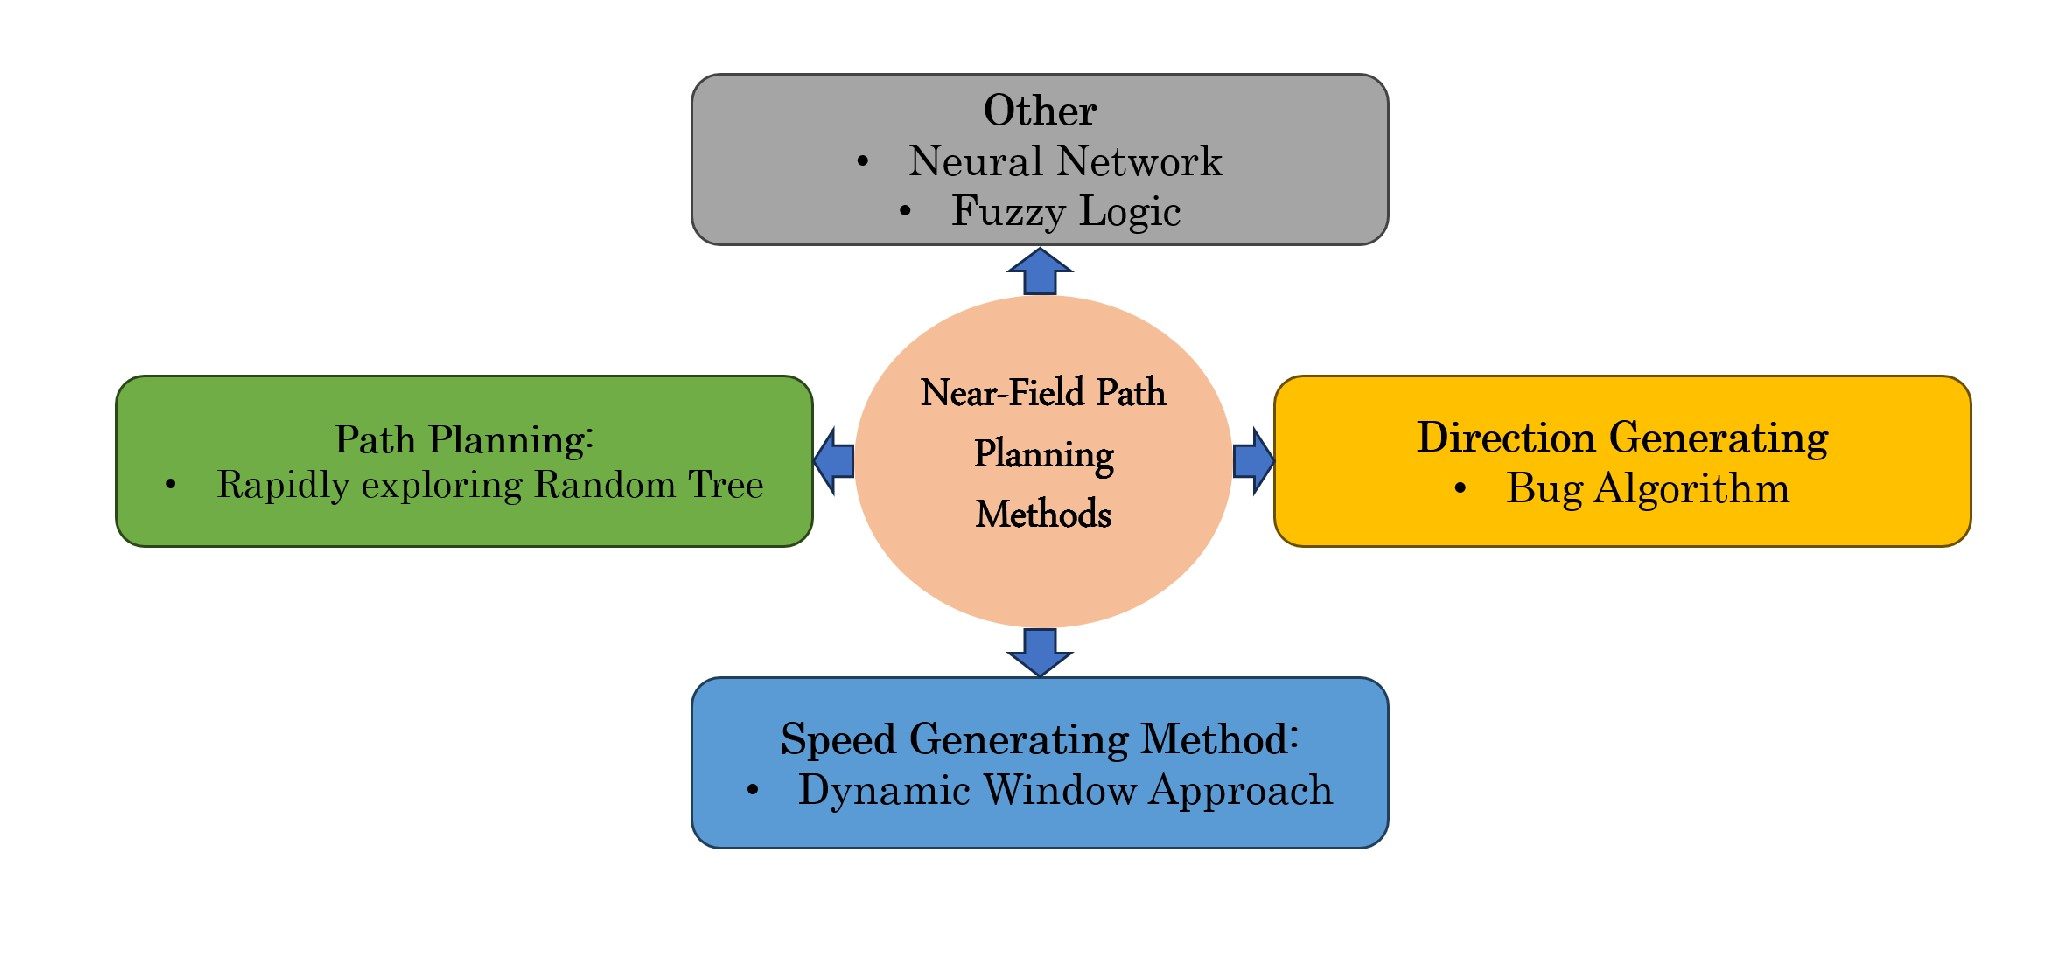
\includegraphics[width=6in]{images/Chap1/PP_Approaches.jpg}\\
        \caption{Clustering Of Near-Field Path Planning Approaches \cite{R28}}
        \label{cluster}
        \end{center}
\end{figure}

The process groups are then differentiated to identify their advantages, limitations and suitability 
to the problem statement. For each cluster one or two methods are studied and explained, through which 
the discrimination is made. 

\textbf{Direction-generating methods} compute feasible travel directions (directional state space) 
based on sensory input, which the AMR should follow in the next time step \cite{R28}.
A very simple algorithm for obstacle avoidance is the Bug algorithm.
In their research paper \cite{R25},
Buniyamin, N. et al. propose the point to point Bug algorithm to navigate in unkown environments. 
Bug algorithms are based on range sensors input. As illustrated by \ref{Bug_Algo}, the robot at the 
starting point (Start green dot), 
plans to move directly to the 
Goal (Goal Red dot). Then it rotates scanning for obstacle points. 
If it encounters a sudden obstacle point \((A)\), it navigates in its direction.
The robot rotates in the target's direction (\(B\) then \(C\)) until it is able to resume its direct path to 
the target based on the 
constant search for the shortest distance from the current standpoint or find the next obstacle. 

While this approach is simple from the computational point of view and the hardware used, it may not be 
optimal considering other metrics. First it can be significantly affected by sensory noises.
Besides, its path length optimality depends on the nature of the environments and the number of obstacles 
and its effciency decreases if the complexity (obstacle density) of the test area increases: in figure 
\Ref{Bug_Algo}, the path rich in vertices : start-A, A-B, B-C, and C-goal, which makes it 
long and lacks optimization.

\begin{figure}[H]
    \begin{center}
        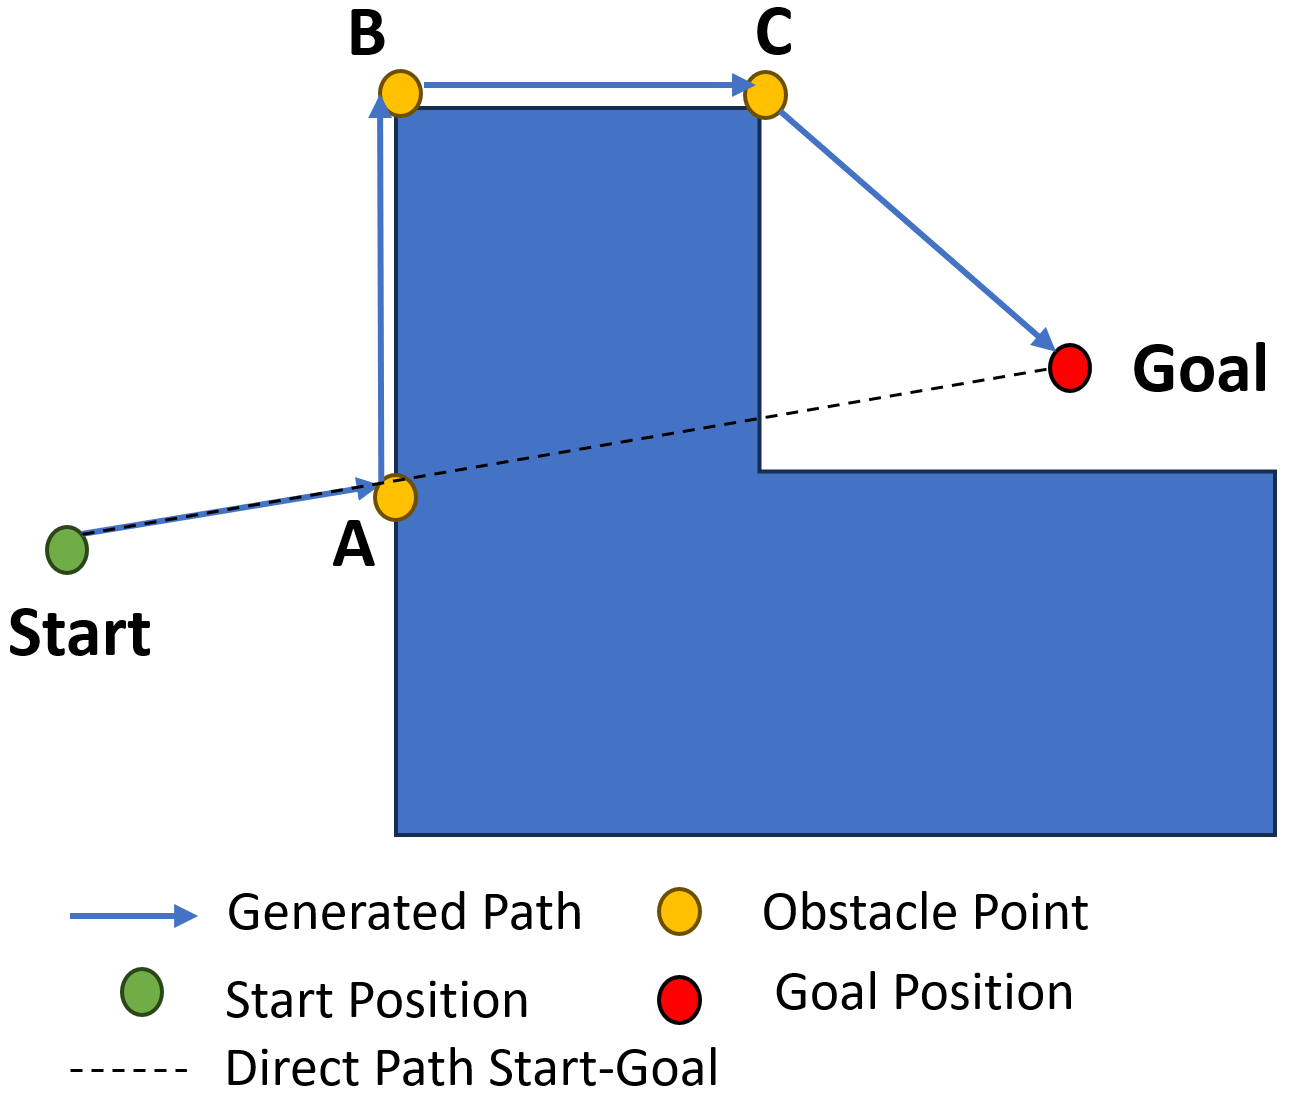
\includegraphics[width=3in]{images/Chap1/Bug_Algo.png}\\
        \caption{Bug Algorithm Path Solution to navigate from Start to Goal while avoiding
        the obstacle}
        \label{Bug_Algo}
        \end{center}
\end{figure}

\textbf{Velocity-generating path planning methods} are algorithms used in AMRs, to calculate both 
the speed and direction of movement. They predict the rotational and translational velocites 
creating the state space of velocities and taking into account the sensory inputs \cite{R28}. 
The Dynamic Window Approach (DWA) is a Velocity-generating path planning method.

In \cite{R19}, Liu et al. used Djikstra ALgorithm (A path-generating Algorithm) 
for Global path planning and 
the DWA as the local path planner for sudden unkown obstacles that could 
appear for smart cars while following the global path.
It works by evaluating different possible movements the robot could make within a short time frame 
and choosing the one that avoids obstacles while also moving towards the goal. The "window" refers 
to a limited set of possible velocities of the velocity space the robot can use based on its current 
speed and capabilities. Figure \Ref{flowchart of the DWA} details the flowchart of the DWA. 

The DWA algorithm starts by analyzing the car's position and base data. It then samples the speed and 
generates a range of possible trajectories. Each trajectory is evaluated to check if it will collide with 
obstacles. If a trajectory is collision-free, it's considered for optimal trajectory selection. This process 
continues until all possible trajectories have been evaluated or an optimal one is found.
The combined algorithms were tested on 3 spaces with 3 stages of environment complexity ranging from 
simple to complex. However, the tests were effected with dynamic obstacles only inside the simulation and
soit is subject for the reality gap problem.
While these methods excel at avoiding obstacles at high speeds, they struggle with local minima. This is 
because they don't consider the overall structure of the free space when evaluating movements.
Additionally, these velocity-generating methods have limitations in mapping the future movements of 
non-holonomic platforms. For example, a method might suggest a movement that is impossible for the 
vehicle to perform due to its non-holonomic nature \cite{R28}.

\begin{figure}[H] 
\centering  
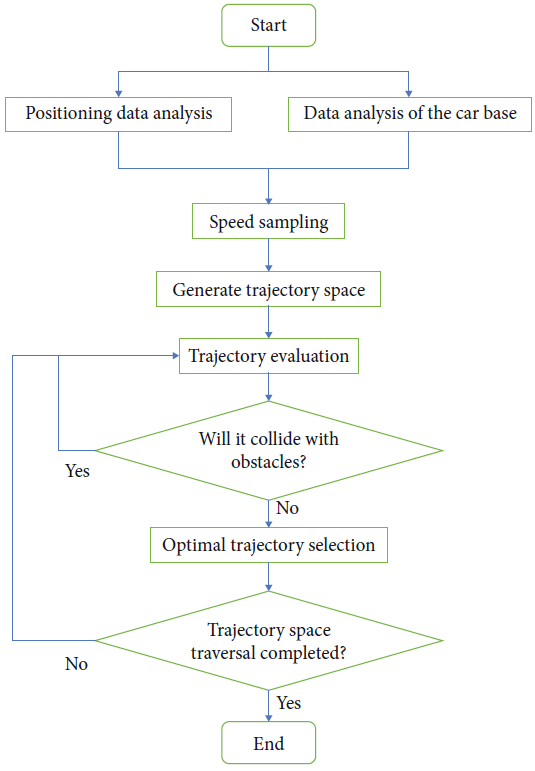
\includegraphics[width=3.5in]{images/Chap1/DWA_flowchart.png}  
\captionof{figure}{Flowchart of the DWA \cite{R19}}  
\label{flowchart of the DWA}  
\end{figure}

\textbf{Path-generating path planning methods} plan entire trajectories in advance, considering both the 
vehicle's position and its intended path over time. These planned trajectories are then combined with 
the previously calculated overall path. Currently, various path planning methods are used in both industry 
and research \cite{R28}.
For example, A* Algorithm is a Path-generating Grid-based method where
the environment is partitioned into a grid of discrete cells, where each cell represents a 
portion of the space. 
The algorithm then traverses these cells to identify suitable paths based on factors such as occupancy 
or cost. For example, in the A* algorithm, the fitness function is calculated from the start point 
to the reached cell, while in the Dijkstra algorithm, it's from the reached cell to the destination. 
While this approach offers a straightforward understanding and implementation, its computational cost 
can be significant due to the large number of cells to evaluate and the repetitive nature of the 
calculations. Additionally, grid-based methods are often constrained by the fixed directionality 
of the grid. The paths generated are restricted to the directions defined by the grid. 
For instance, if the grid is aligned along the x and y axes, the robot can only move horizontally 
or vertically. This can be inefficient or even impossible in environments where diagonal 
or more complex movements are required.
On the Other hand, 

Lavalle \cite{R47} created a method called Rapidly-exploring Random Trees (RRT), a randomized data structure used 
for various path planning tasks. It starts with a single node (usually the starting point)
and iteratively grows a tree by adding new nodes. At each iteration, a random point is sampled from 
the search space. The nearest node in the tree is found, and a new node is added along the path to 
this random point. This process is repeated until a path is found or a maximum number of iterations 
is reached. RRT is particularly effective for exploring complex environments with obstacles. 
Figure \Ref{sampling-based}, illustrates the test of RRT in an obstacle-rich environment (shown in blue)
using 1, 4, then 32-core processors. The planned paths (branches) are shown in grey. 
The path calculated as optimal is shown in red and connects the start pose with the goal pose.
These algorithms present advantages like handling big environments and complex obstacle
situations, however, they can also be computationally intensive and demanding in complicated situations.
Figure \Ref{sampling-based} shows the difference in the resulting optimal path in a cluttered environment where with
1 core the algorithm successfully finds a feasible path, and, as the cores double, the computed path
improves its quality as the search tree expands. 
RRTs require collision checks for each new node, which can be computationally expensive and memory-intensive, 
especially in environments with numerous obstacles, heavy traffic, or complex paths.


\begin{figure}[H]
    \begin{center}
       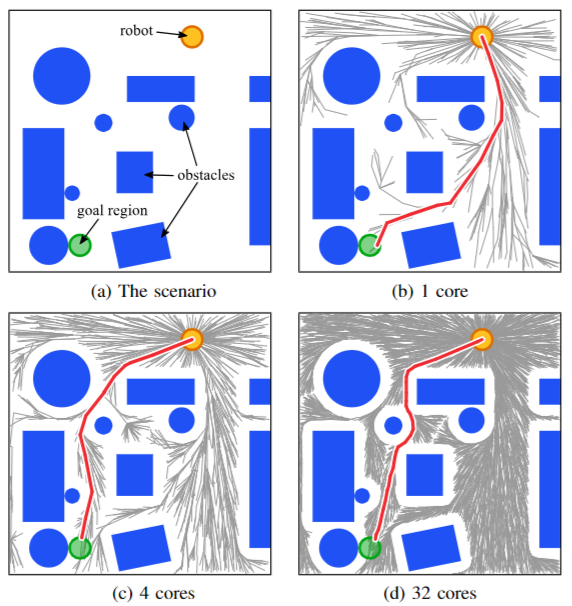
\includegraphics[width=3.5in]{images/Chap1/sampling-based.png}\\
       \caption{RRT ran on a non-holonomic robot using 1, 4, then 32-core 
       processors \cite{R16}}
       \label{sampling-based}
       \end{center}
\end{figure}

\textbf{Artificial Intelligence-based methods} 
leverage the use of Neural Networks, Fuzzy Logic, Reinforcement Learning, and Evolutionary algorithms. 
These methods learn from experience, adapt to changes, and optimize paths in complex environments. 


To start with, Neural Networks (NN) are inspired from the biological harmonious connection of the brain neurons
that gives it the ability to process big amounts of data and generate ideas and decisions and solve problems. 
The NN is built in a way that enables it to get its input in a form of data and process it by learning, improving 
and adjusting the output to the desired results. NN are able to perform Parallel processing: the information is 
transmitted in two
directions to the neuron in the case of Recurrent Neural Networks (RNN) that allows for learning fron current and 
past inputs to the NN. This approach improves the computation time and overall performance. 
The NN is then able to process solutions that create paths for difficult environments. 
However, it presents a practicality challenge. Although the performance an results can be impressive, yet, in a 
real-time context, 
it is unfeasible to rely on solutions that require extensive computational efforts and need long durations to 
process solutions. In addition, the number of neurons and layers have to be scalable and depends closely on the 
level of complexity that the vehicle is to deal with: NN are trained using a usecase so the 
outcome is tightly related to that use case and is not as efficient in other applications \cite{R12}. 

On the other hand, Reinforcement Learning (RL) can be used to learn optimal paths by interacting with the environment. 
The robot learns a policy that maximizes cumulative rewards, where rewards are given for reaching the goal, avoiding 
obstacles, and minimizing path length. The policy is often represented by a neural network, and the path is optimized 
as the robot learns from its experiences. Reinforcement learning (RL) methods for path planning in wheeled mobile robots 
face significant limitations due to high computational costs and long training times. These methods require extensive 
data to cover various scenarios, making the process time-consuming and resource-intensive. Training an RL agent, 
particularly in complex environments, can take millions of interactions, which is impractical for real-time applications. 
Additionally, as the environment's complexity increases, the state and action spaces expand, 
leading to scalability issues and longer training times. When combined with deep learning, RL becomes even more 
computationally demanding, requiring substantial resources and careful tuning of hyperparameters.

Fuzzy Logic (FL), on the other hand, is a way of thinking that mimics how humans make decisions, especially when things are unclear 
or uncertain. Instead of working with exact numbers, it uses "fuzzy" terms like "good", "average" or "bad" to make 
decisions. Input numbers are clustered following the fuzzy sets or intervals and assigned a value using membership 
functions. Later the values are interfered and defuzzified to genearte the ouput as a command value. 
In robotics and path planning, FL helps robots navigate by allowing them to handle uncertain situations, 
like avoiding obstacles or finding the best route, even when the environment is not fully known. Instead of needing 
exact data, the robot can employ fuzzy terms like "close" or "far" to understand its surroundings. For example, if an 
obstacle is "somewhat close," the robot can smoothly adjust its path to avoid it. FL also helps the robot choose the best 
route by weighing factors like distance, even when the information is not fine-tuned. This improves the 
robot's handling of dynamic environments and making flexible and optimal decisions.
However, one 
disadvantage is that it can be tricky to create the right rules for the robot to follow, and the system can become 
complicated as more rules are added. It may present a scalability problem because in unpredictable and dynamic environments
it is not evident to overfit fixed fuzzy sets to be practical in all of the cases \cite{R12}.

While Neural Networks and Fuzzy Logic offer powerful approaches for handling uncertainty and complex decision-making, 
another key area in artificial intelligence for path planning is the use of meta-heuristic algorithms.
Meta-Heuristoc algorithms are inspired from biological and natural processes for evolution and survival. 
Relying on environmental input like obstacles and targets, meta-heuristic algorithms explore the solution
space by evolving random solutions for the problem and optimizing them by rounds until a stopping criterion or set
of criteria is satisfied (see more in section 4: Heuristic Approaches).
Approaches like Genetic Algorithms (GA) have been used for path planning by Ahmed Elshamli et al. \cite{R17}. The The robusteness of their 
solution is its adaption to dynamic environments. They evolve their GA using variable size chromosomes, where each node 
represents a waypoint of the path, then they measure the quality of each path using an evaluation function. A modified Genetic Approach is then 
applied to each population: Crossover, mutation, \textbf{Repair} infeasible paths, \textbf{Shorten}, then \textbf{Smoothen} 
feasible paths while dynamically checking for new obstacles.
The approach is tested in static and dynamic environments and has achieved proven efficiency when it comes 
to local optima challenges and survivig the best elements of the population. While the use of the GA itself is robust
and successful, it can be challenging to recreate the algorithm and to add the improvements. In addition, the tests
the ran are limited to a simple simulation with unrealistic situations and obstacle setting as displayed in 
figure \Ref{R17 test scenarios}: In reality, the hardware used to detect surrounding objects are scan based sensors
for instance LiDAR. They scan \(360^{\circ}\) of the surrounding starting from the robot as the origin.
This scan provides a polar perception of the obstacles (see figure \Ref{scamSim}). 
A polar perception only renders the perceivable surface of the objects.
The objects' depth and dimensions are not available through this sensorial input.
Obstacle perception is challenging due to limited knowledge of their exact contours and the 
discrete nature of optical sensor scanning. Connecting perceived points to form closed contours can 
be ambiguous, especially at a distance.

\begin{figure}[h!]
    \centering
    \begin{minipage}{0.30\textwidth}
        \centering
        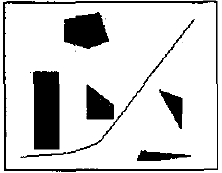
\includegraphics[width=\linewidth]{images/Chap1/R17_simple.png} % Replace with your figure
        \caption{Simple obstacle environment       }
        \label{Simple obstacle environment}
    \end{minipage}
    \begin{minipage}{0.30\textwidth}
        \centering
        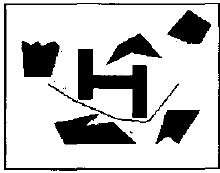
\includegraphics[width=\linewidth]{images/Chap1/R17_intermediate.png} % Replace with your figure
        \caption{Intermediate obstacle environment}
        \label{Intermediate obstacle environment}
    \end{minipage}
    \begin{minipage}{0.30\textwidth}
        \centering
        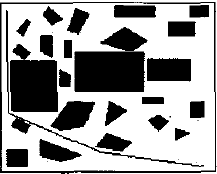
\includegraphics[width=\linewidth]{images/Chap1/R17_complex.png} % Replace with your figure
        \caption{Complex obstacle environment}
        \label{Complex obstacle environment}
    \end{minipage}
    \caption{GA Test scenarios \cite{R17}}
    \label{R17 test scenarios}
\end{figure}

While Classic path planning methods (Path-generating, Velocity-generating, and Direction-Generating) 
have proven effective across various applications and usecases, 
they often face challenges when applied to highly structured, repetitive environments like those found 
in industrial automation. To overcome these limitations, the research in the previous years became rather 
oriented to investigating and using heuristic approaches. In \cite{R26}, Masehian et al. conducted a 
chronological review about the followe approaches in Motion Planning (MP). The results testify that in 30 years,
The application of Heuristic approaches in MP went from 0\% to 54\% from 1977 to 2007 as shown on Figure 
\Ref{heuristic barchart}.

\begin{figure}[H]
    \centering  
    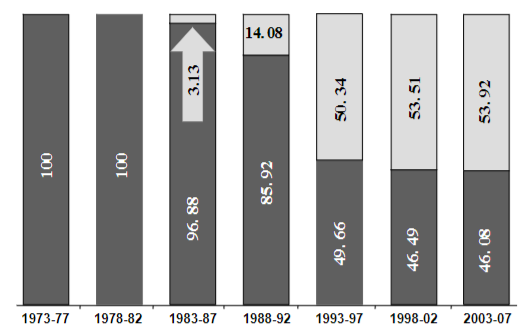
\includegraphics[width=3.5in]{images/Chap1/heuristic_barchart.png}\\ 
    \captionof{figure}{Application of classic and heuristic approaches in MP \cite{R26} 
    \newline \textbf{Dark gray:} Classic approaches
    \newline \textbf{Light gray:} Heuristic approaches }
    \label{heuristic barchart} 
\end{figure}

To draw to a close, even though the heuristic approach prevails the classic one:
\cite{R20} and \cite{R25}, these approaches are not without their limitations. Heuristic methods, while good at 
navigating complex environments and avoiding local minima, sometimes fall short in finding the best possible 
solutions, especially in high-dimensional spaces.

\subsection{Discussion: Selection of the Path Planning Method}

Path-generating methods are particularly promising for intralogistics applications involving autonomous 
mobile robots (AMRs). Unlike direction-generating methods, these methods are well-suited for dynamic environments. 
These methods effectively handle dynamic environments and disturbances while minimizing oscillations and 
computational costs.
They can also incorporate kinematic constraints and generate optimal trajectories in complex, unstructured areas. 
Compared to speed-generating methods, path-generating methods allow for dynamic planning horizons, enabling the 
calculation of optimal routes that avoid dynamic obstacles and disturbances. Given these advantages, this work 
will focus on path-generating methods for subsequent developments.


To enhance the efficiency and effectiveness of path planning, innovative approaches are emerging. 
By combining traditional methods with cutting-edge optimization techniques, we can overcome the 
computational challenges and achieve more robust solutions. These hybrid strategies offer a 
promising path forward, paving the way for advancements in path planning technology.



\section{Heuristic Approaches}
%intro
This section will focus on the Application of heuristic algorithms for solving robotic path planning 
problematics. 

\subsection{Optimization Techniques}
Optimization refers to the decision making led by the machine with availability of certain circumstances and constraints
thet either help or limit the outcomes of the optimizer \cite{R37}. In the case of path planning, optimization aims
to modify some properties of the generated solutions to cope with the surrounding conditions.
In stochastic environments, it is challenging to plan feasible paths given the high dynamics 
and obstacles.
The increase in the complexity of the environment and the constant dynamics increase the number of variables involved 
in the mathematical representation of the problem. As a consequence, it raises the computation efforts that need to be 
deployed for the creation and optimization of the solution and decreases feasibility \cite{R7}.
In order to get optimal results like smooth and short paths, finding a feasible path is not enough. The evaluation 
of the generated path and the optimization are helpful to ensure that the robot is driving the optimal path.
There exists a range of planners and optimizers which are clustered as classic and Heuristic approaches \cite{R12}.
Classic approaches include \textbf{Analytical} and \textbf{Enumerative} methods. 
The former rely on mathematical modeling, which can become unsolvable as the navigation environment becomes more 
cluttered. Additionally, applying these models can be challenging in scenarios where the necessary models for different 
components are not readily available. The latter have the drawback of increased intricacy in bigger or more elaborate 
search spaces. On the other hand, Heuristic approaches can be sub-categorized into \textbf{Meta-Heuristic} and \textbf{Evolutionary algorithms}.
Some of these methods can fall in the trap of local minima and sub-optimality \cite{R12}
Alternatively, sebsequent to a review of the available planning and control approaches in intralogistics, Fragapane, G. et al. \cite{R7}, 
concluded that nature-inspired algorithms can instill intelligence into planned paths.
Elshamli, A. et al. explained in \cite{R17}, that Meta-Heuristics are adaptive to the dynamics of the surroundings
unlike classic approaches that proceed sequentially to generate solutions. The paths developed by classic approaches
can thus become infeasible in a later stage if the environment changes. Metaheuristic approaches are based 
on parallel search mechanisms that can have updated input of the conditions and thus are more adaptive and 
practical in real-world scenarios.

Next, this section dive into Meta-Heuristics which are defined by Bilal et al. as 'the optimization
techniques mainly based on function evaluation and make little
or no use of the properties of objective functions and constraints.
Meta-heuristics are thus problem independent techniques not taking
advantage of any specificity of the problem’ in their review \cite{R37}.
The authors later break down Meta-Heuristics into \textbf{Neighborhood-based Algorithms} and \textbf{Population-based Algorithms}
as given by the tree graph in Figure \ref{Tree}

\begin{figure}[H]
    \begin{center}
        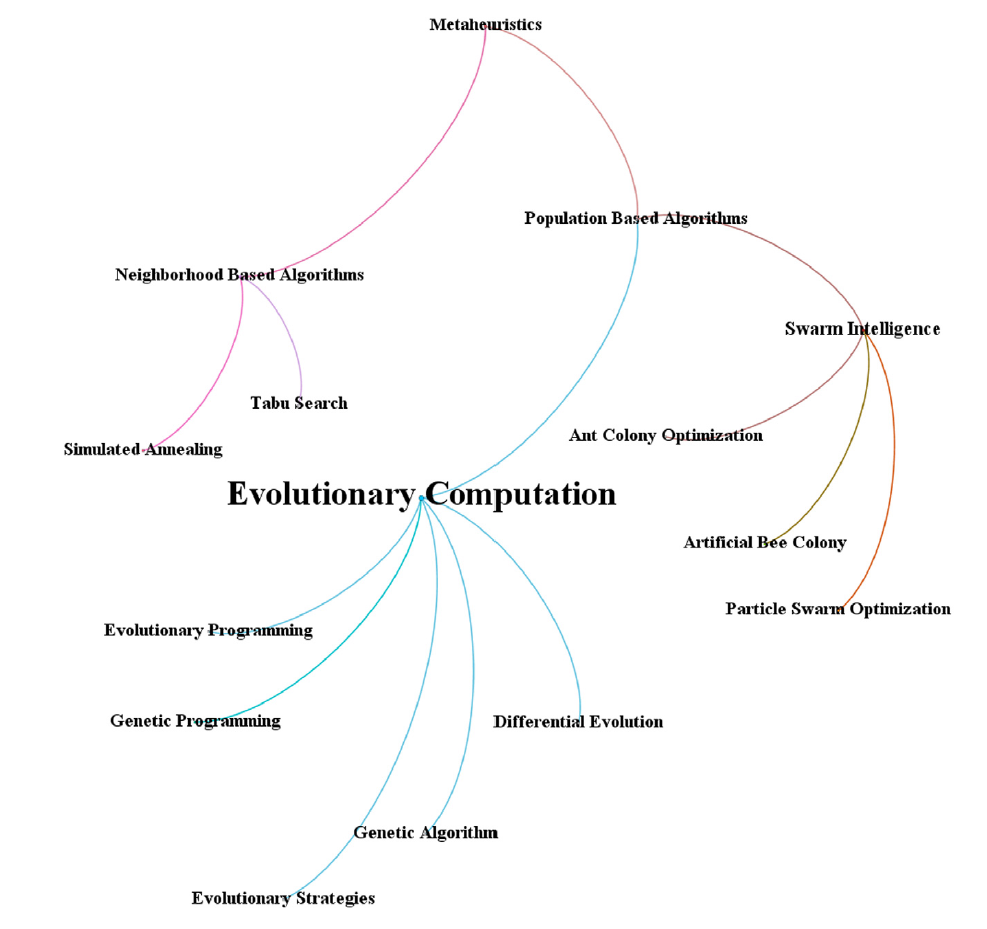
\includegraphics[width=\linewidth]{images/Chap1/Tree_Metaheuristic.png}\\
        \caption{Tree of Meta-Heuristic Algorithms \cite{R37}}
        \label{Tree}
    \end{center}
\end{figure}

The Neighborhood-based algorithms benefit from the neighboring solutions by migrating from the current solution to 
the near surrounding solutions with the goal of improving the fitness function. The examples mentioned for this 
approach are Simulated Annealing (1979) and Tabu Search (1989). The Population-based algorithms are methods that start from a sample population and rely on their evolutions. 
They are inspired by the evolutionary processes observed in nature and are sub-categorized in this approach under 
Swarm intelligence and Evolutionary Algorithms. 
Swarm Intelligence approaches are analogous to the socio-cooperative practices of species like bees, ants, and birds. 
For instance, Ant Colony Optimization (1992)and Particle Swarm Optimization (1995) are examples of such algorithms. 
On the other hand, Evolutionary algorithms rather copy the species evolution theory, among which are Differential 
Evolution (1995) and Genetic Algorithm (1957) \cite{R37}.

Metaheuristics, mainly Swarm-based methods and Genetic Algorithms, 
have been used multiple times for robotic path planning, as noted in the literature. 
Each algorithm has its own unique search methods and strengths, providing different benefits and 
areas for optimization.
  


\begin{figure}[H]
    \centering
    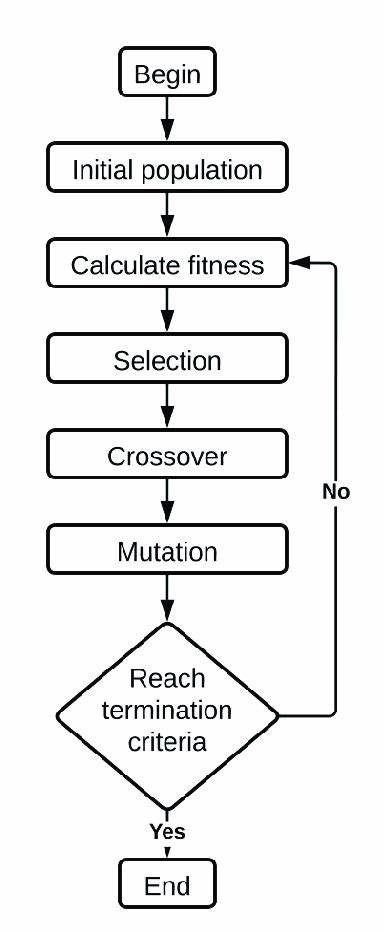
\includegraphics[width=2in]{images/Chap1/GA.jpg}
    \caption{Flowchart of the GA \cite{R39}}
    \label{GA}
\end{figure}

Elshamli, A. et al. \cite{R17} have employed the Genetic Algorithm (GA) (See algorithm steps in figure \Ref{GA}) to solve 
the problem of path planning in dynamic environments. They represent their paths using chromosomes where each node of the chromosome represents 
a waypoint and develop a variable chromosome length approach that accommodates obstacle avoidance and efficiency 
in reaching the goal. The fitness of each chromosome is evaluated according to an objective function that includes path length, smoothness, 
and clearance to obstacles. A modified genetic Algorithm is applied where after crossover and mutation, paths are 
shortened and smoothed if it is possible. Saving the best individuals generated by the GA was effective in delivering the overall best solutions.
Tamilselvi, D. et al. also modified the GA by applying the elitism concept. 

This is achieved by saving the best individual, denoted as \(S_{best}\), and replacing the worst individual in the 
next generation with \(S_{best}\). This approach helps to prevent premature convergence to local optima, increasing 
the likelihood of finding the global optimum. In the context of path planning, elitism has proven effective 
in discovering feasible paths in environments with limited dynamic obstacles. Additionally, by incorporating 
a motion prediction mechanism based on the grid map, elitism can be adapted to handle dynamic obstacles more 
effectively \cite{R38}.

Authors of \cite{R40} also worked on the path planning in dynamic environments problem. They crtic the GA to be computationally
intensive and to require long planning time. Instead they suggest the Simulated Annealing algorithm (SA)
to solve the path finding problem. 

\begin{figure}[H]
    \centering
    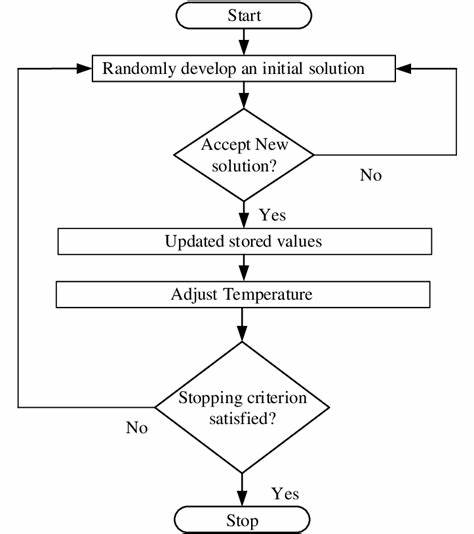
\includegraphics[width=3.5in]{images/Chap1/SA.jpg}
    \caption{Flowchart of the SA \cite{R41}}
    \label{SA}
\end{figure}

Being a probabilistic meta-heuristic algorithm it is designed to guide the local
optimum to a global optimum. The approach is based on the evaluation of the path length to discriminate 
path candidates: the shorter the path the better. It works by trying out different paths for the robot, beginning 
with a high "temperature" that lets the algorithm accept good paths and bad paths with a accepted with a certain probability,
which decreases over time (simulating the cooling process in annealing). This helps it explore a wide range of 
options and avoid getting stuck in a local minima . As the process continues, the temperature slowly decreases, 
making the algorithm less likely to accept bad paths, and helping it to focus on finding the global minima as given by 
figure \Ref{SA}. algorithm was tested in four environments with different static and moving obstacles. The algorithm 
successfully found the best or nearly best paths and could quickly adjust to avoid collisions in real-time. 
Compared to a genetic algorithm, the SA method was 57\% faster for complex environments and 74\% faster for simple
environments. However, the processing time increases exponentially for complex environments (13.57 seconds).

Particle Swarm Optimization Algorithm (PSO), as well, is used for solving non-linear optimization problems like scheduling, power 
management and also robotic path planning. It is inspired from the cohesive behavior of bird and fish swarms traveling 
together.It works by having a group of particles (potential solutions) move around in the search space to find the best 
solution. Each particle in the PSO algorithm remembers the coordinates of the best solution it has found so far, known 
as its personal best (pbest). Additionally, the algorithm tracks the best solution found by any particle, referred to as 
the global best (gbest). The core idea of PSO is to guide each particle towards both its pbest and the gbest positions:
from state a to c as given by figure \Ref{pso}, 
using a randomly weighted acceleration during each iteration. The algorithm iteratively updates the particles' positions 
and velocities until an optimal or near-optimal solution is found.
Alaliyat, S. et al. have investigated dynamic environment navigation using PSO. They found out that the performance 
of the algorithm depends on parameters tuning. Overall, feasible paths were successfully generated.
Planning time is rather high for simply organized environments (18.35s) and higher for the most complicated scenario
(31.17s).

\begin{figure}[H]
    \begin{center}
        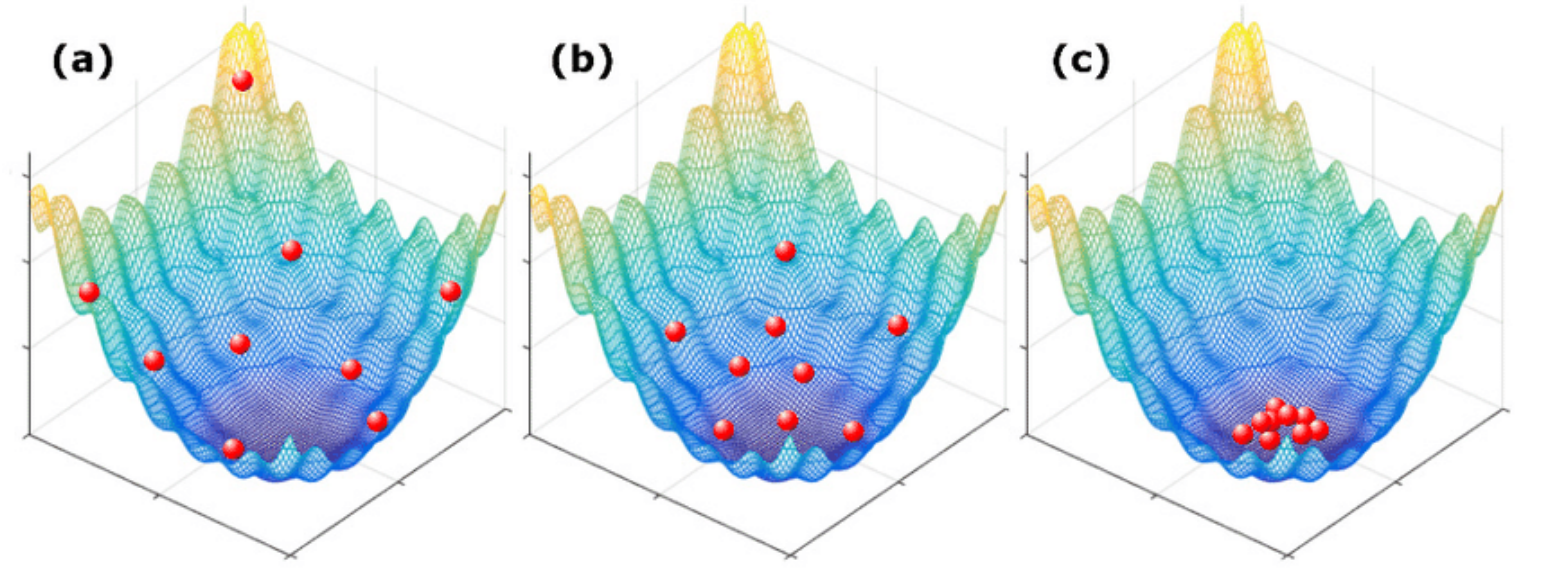
\includegraphics[width=4in]{images/Chap1/PSO.png}\\
        \caption{Particle Swarm Optimization \cite{R42}}
        \label{pso}
    \end{center}
\end{figure}

Defferential Evolution (DE) has been used in a hybrid algorithm along with PSO by Tand, B. et al. \cite{R43} to leverage 
both of the algorithms benefits. DE is rarely solely applied to path planning problems. In their review \cite{R37}
, of 20 years of research about DE, Bilal et al. did not mention robotics among the fields of application of DE. 
DE starts with a set of potential solutions. Each solution, or individual, is modified 
through mutation, crossover, and selection to improve over time. Mutation introduces random changes to create new 
candidates and avoid getting stuck in local optima. Crossover mixes parts of the new candidates with the original 
solutions to explore new possibilities. The selection process keeps only the better solutions for the next generation. 
This method effectively balances exploring new options and refining existing ones, making DE well-suited for complex 
optimization tasks.
By integrating improved PSO and DE algorithms for enhancing particle diversity, Tand, B. et al. achieved better 
path quality compared to other methods. The results demonstrate that their approach outperforms traditional 
evolutionary algorithms in path optimality an optimize computation times by 1.38\% \cite{R43}. 

Ant Colony Optimization (ACO) is known for being robust and good at parallel processing, but it can be slow and 
sometimes gets stuck in local optima solutions. To fix this, improvements like Ant Colony System (ACS) 
and Max-Min Ant System (MMAS) have been developed, which make ACO better at finding solutions but still have 
issues like being too rigid and converging too early. In mobile robot path planning, new strategies have been 
created to address these problems, such as adaptive methods that improve how pheromones are updated and balance 
exploration with finding the best path. Recent research has also introduced advanced versions like polymorphic 
ACO and multi-objective optimization, making ACO more effective for real-time and complex situations. However, 
these improvements also make the algorithm more complex and take more time to compute.

%advantages & limitations in discussion:

Meta-heuristic algorithms, such as Genetic Algorithms (GA), Particle Swarm Optimization (PSO), and Differential 
Evolution (DE), have become increasingly popular in robotic path planning. These algorithms are attractive because 
they can find good solutions to complex problems by mimicking natural processes like evolution or swarming behavior.
However, despite their growing use in research and their potential efficiency in practical usecases, the application 
of meta-heuristic algorithms in real-world robotic path planning like the intralogistics field remains quite limited. 
One of the major issues is that most studies focus on simulations rather than 
testing in real environments. While simulations can help develop and adjust these algorithms, they do not fully 
cover the challenges robots face in the real world, such as varying conditions, surface types, or unexpected 
noises. Another major issue is how obstacles are represented in these studies. Often, obstacles are either unrealistically 
large compared to the robot or have overly simple shapes that don’t accurately reflect real-world conditions. This 
lack of realism can result in algorithms that work well in simulations but fail when used in real environments. Additionally, 
because these algorithms are mostly tested in controlled, simulated settings, they may be too finely 
tuned to those specific conditions. This can make them less reliable when applied to the unpredictable conditions 
of the real world gap. In summary, while meta-heuristic algorithms show promise for robotic path planning, more real-world 
testing and realistic obstacle modeling are needed to ensure they work effectively in practical situations. 
Addressing these issues is key to advancing the use of robotics in intralogistics and other fields.
\newpage
\section{Discussion} %TODO: change name it is soa here
To synthesize the research conducted, it is paramount to summarize the \textbf{key concepts} comprehensively and 
pont out the general \textbf{drawbacks}. This 
State of the Art report focuses on mobile robot path planning, a critical component of the overall 
robotic planning process. Effective path planning not only organizes and optimizes a robot's navigation 
but also significantly enhances its productivity by enabling it to execute missions more efficiently. 
In dynamic environments, a well-designed path planner is essential for ensuring safe operations and 
maximizing the robot's resource utilization and operational capacities.
Meta-heuristic optimization algorithms are highly effective for refining mobile robot paths, particularly 
when building routes from scratch while considering both static and dynamic obstacles.
They also have the capability to solve problems without information about their mathematical model.
This has the great advantage of reducing the burden of expliciting the situation in order to solve it especially 
in complex cases where the effort to model the problem and the contsraints is higher and, later, the computation 
is harder. Instead, meta-heuristic algorithms focus on optimizing the fitness function related to the specific 
usecase. 

The path planning methods discussed have several drawbacks. Grid-based methods can be easily misled by noisy 
sensor data, and their generated paths might not be the shortest possible, particularly in crowded areas. 
Some methods excel at high speeds but struggle with dynamic environments, while others may have limitations 
in planning for non-holonomic vehicles. Computational efficiency is a concern, as some methods are slow and 
resource-intensive, especially in complex environments. Heuristic methods, while effective, might not always 
find the optimal solution. Real-world applications pose additional challenges. In dynamic warehouse settings, 
blocking areas for extended path planning can disrupt operations, interfere with other vehicles, and reduce 
productivity. Metaheuristic optimization approaches have been limited to mission scheduling in intralogistics 
robotics, with fewer applications in path planning. Addressing these limitations requires innovative solutions 
that balance computational efficiency, real-time performance, and path quality.

Furthermore, the classical and the heuristic approaches are capable of creating new different paths every time the 
algorithms are ran even in the same environment setting. While this phenomenon proves of the intelligence of the algorithms
and the availability of several optimal paths, it makes the fully automated robot's behavior non-repeatable and unexplainable. 
For humans, it is difficult to foresee the behavior if many options are available. However, it is important for those working 
closely to robots to have an expectation of their behavior. It enables them to avoid collision risks and injuries and to 
plan their actions accordingly. If a predictable vehicle behavior is available, it promises a structured approach to path 
generation, reducing computational complexity and improving path quality.

Combining an optimal path planning approach that accomodates the kinematic constraints of Autonomous forklifts in the
intralogistics environment and generates smooth paths, is behaviorally explainable and deploys meta-heuristic 
Algorithms is a new approach that would have an added value to mobile robot path planning in Intralogistics of 
reducing computation time and travel distance and improving AI driven solutions explainability. 

\section{Adopted Path Planning and Optimization Methods}

The obove discussed Path Planning approaches are typically
designed to solve path planning problems in various environments and have been used in multiple
applications.
For this project's problem, the robot operates in a consistent environment—the station. 
Although stations may differ in 
position, size, and layout, the components within them remain the same: shelves containing pallets. 
This consistency suggests that we should 
develop a solution specifically tailored to the station environment, which would help minimize potential problems 
and reduce the effort required to solve them. 

A path planning module has already been developed at STILL for the autonomous 
forklift trucks, utilizing classic sampling-based path planning methods. This module is based on the Open Motion 
Planning Library (OMPL), an open-source library for motion planning in robotics. OMPL is designed for complex use 
cases and includes several algorithms, such as probabilistic roadmaps (PRM) and rapidly-exploring random trees 
(RRT), along with their variants. OMPL performs well in clean environments without obstacles, with a minimum 
processing time of \(200ms\) , but in complex environments, processing time can increase to \(2s\).
While it can be very fast in the abscence of obstacles this approach presents some limitations:
\begin{itemize}
    \item Not Station-Specific: While OMPL is a versatile and powerful motion planning library, its general-purpose 
    nature can be a limitation for station-specific pickup/drop operations. OMPL is designed to handle a wide range 
    of environments and tasks, but it may not be as efficient or tailored to the specific constraints and 
    requirements of station-related operations. OMPL may not have built-in knowledge or optimizations for tasks 
    like docking at specific stations, handling different station configurations, or considering constraints 
    related to station-specific equipment.

    \item Too Complex for Simple Tasks: OMPL's advanced algorithms, while powerful, can be overkill for simple tasks 
    like pallet handling. Its general-purpose nature can also lead to computational overhead, 
    especially in less complex environments. This suggests that tailoring OMPL to specific station-related 
    operations could improve its efficiency and effectiveness.
    
    \item Long Processing Time: OMPL's processing times can be substantial, particularly in complex environments 
    with numerous obstacles, tight spaces, or frequent changes in the environment. 
    This can lead to delays in decision-making and potentially hinder the overall efficiency of operations. 
\end{itemize}

Given OMPL's limitations, I propose a station-based approach is needed. This approach will be tailored 
to the structured environment of the station, enabling faster and more efficient path planning. 
By minimizing directional changes and adhering to station boundaries, we can achieve shorter and repeatable 
path calculation times, optimizing the overall efficiency of operations. By focusing on the typical tasks of pallet 
pickup and drop-off, we can create a solution that works effectively in simple and moderately complex 
situations, reducing processing time and resource usage. 

For optimizing paths, various approaches exist.
Path optimization can be approached mathematically using Jacobians, which map control inputs, like position or wheel 
speeds, to the desired outcomes. The objective is to minimize a cost function—such as path length, energy use, 
or time—by adjusting the robot's control inputs to achieve the desired position. A common technique is gradient descent, 
where control inputs are iteratively updated to reduce the cost. The Jacobian matrix, which links these 
inputs to the robot's position, guides these adjustments until the most efficient path is found. However, the Jacobian-based 
optimization method poses several challenges for this use case. For wheeled mobile robots with multiple control inputs, 
the Jacobian matrix can become complex and large, leading to increased computational costs and making real-time 
optimization challenging. 

Frequent updates in dynamic environments further add to this load, potentially leading to delays or suboptimal paths. 
Mukherjee et al. \cite{R44} noted that their approach to optimal trajectory planning does not guarantee a global 
optimum but rather an isolated local optimum close to the global one. Additionally, this method relies on precise 
kinematic and dynamic models, so any inaccuracies, such as sensor errors, can result in poor path optimization. 
In this context, the kinematic model would need to be refined for the specific truck using it. Managing complex inequality 
constraints, like obstacle avoidance, can also complicate the optimization process and reduce efficiency.

Reinforcement Learning (RL) offers a promising approach to learning optimal paths for mobile robots. By interacting 
with the environment and maximizing rewards, RL agents can develop effective policies. However, RL methods for 
path planning in wheeled mobile robots face significant challenges, including high computational costs, long 
training times, and the need for extensive data. These limitations make RL impractical for real-time applications 
in complex environments.

As highlighted in the previous Section , meta-heuristic approaches, though powerful for solving complex problems, 
often require significant computational time. However, this can be greatly reduced by optimizing how these 
methods are applied. Instead of generating a path entirely from scratch, this work proposes starting with a pre-built 
or partially constructed path provides a solid foundation. Additionally, reducing the number of waypoints 
can streamline computation, allowing the algorithm to focus on refining an already good solution rather 
than calculating every detail from the ground up. This approach preserves the strengths of meta-heuristics 
while significantly speeding up the planning process, making it more practical for real-time or near-real-time 
applications.

\section*{Conclusion}

In this chapter a detailed State of the Art related to Intralogistics, AMRs, Near-Field Planning, and Heuristic 
Optimization was laid out. The investigation of the literature helped to address the advantages and limitations
of individual approaches and decide around the relevant approaches to the Problem Statement. 
A Choice of the methodology was conducted at the end taking into account the compiled information.
In the following chapter, we will delve into the design and development of the solution 
combining a Path generating to Metaheuristic Optimization to obtain an optimal path.

